\chapter{Odds, Likelihood and the Weight of Evidence}
\label{ch:odds}

\section{The likelihood ratio as the currency of evidence}

The odds form of Bayes' rule, equation \eqref{eq:oddsform}, says that evidence acts on beliefs by multiplication. Whatever the prior odds of a proposition, evidence $E$ multiplies them by
\begin{equation}
\LR(E) = \frac{\Prob(E \given \Hp)}{\Prob(E \given \Hd)},
\end{equation}
where $\Hp$ and $\Hd$ are the propositions advanced by the prosecution and the defence, or by claimant and defendant. Three features of this formula explain why forensic scientists have adopted the likelihood ratio as the proper measure of the value of evidence \citep{aitken_taroni2004,evett1998}.\index{likelihood ratio}

First, the likelihood ratio is comparative. It does not ask how probable the evidence is in some absolute sense, but how much more probable it is under one account than under the other. Evidence that is equally probable under both accounts, however striking, has a likelihood ratio of one and should not move the fact finder at all. A defendant's nervousness under police questioning is common among the guilty and among the innocent who fear being disbelieved; its likelihood ratio may be close to one even though it feels incriminating.

Second, the likelihood ratio separates the role of the expert from the role of the fact finder. A DNA analyst can say how probable the observed profile is if the defendant left the stain and how probable it is if an unknown person did. The analyst cannot, without trespassing on the jury's function, say how probable it is that the defendant left the stain, because that depends on all the other evidence. The likelihood ratio is exactly the part the expert can speak to.

Third, likelihood ratios for independent items of evidence multiply, so their logarithms add. If $E_1$ and $E_2$ are conditionally independent given each hypothesis, then
\begin{gather}
\LR(E_1, E_2) = \LR(E_1)\,\LR(E_2),\\
\log \LR(E_1,E_2) = \log\LR(E_1) + \log \LR(E_2).
\end{gather}
Good, following Turing, called $10\log_{10}\LR$ the weight of evidence in decibans \citep{good1950,good1979}. A deciban is roughly the smallest change in belief a person can perceive. Ten decibans is a factor of ten, twenty is a factor of a hundred (Figure~\ref{fig:scale}). The additive scale makes it natural to think of a trial as a ledger in which each item of evidence adds or subtracts weight.\index{deciban}\index{weight of evidence}

\begin{figure}[ht]
\centering
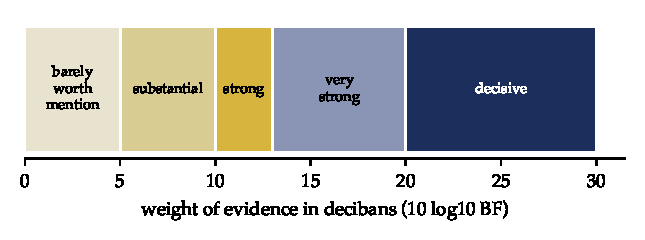
\includegraphics[width=\linewidth]{fig_scale}
\caption{A verbal scale for the weight of evidence, in decibans, in the tradition of Jeffreys and Good. The phrases used in forensic reporting differ in detail.}
\label{fig:scale}
\end{figure}

\section{The fallacies}

Most of the famous statistical errors in criminal trials are failures to distinguish $\Prob(E\given \Hd)$ from $\Prob(\Hd\given E)$, or failures to use the right $\Hd$.

\subsection{The prosecutor's fallacy}

The prosecutor's fallacy, a name due to Thompson and Schumann, is the transposition of the conditional \citep{thompson1987}. An expert testifies that the probability of a random person matching the crime stain is one in a million. Counsel, the judge or the jury then treats this as the probability that the defendant is innocent. The two are entirely different. In a city of ten million, about ten people would match. If there is no other evidence pointing to the defendant, the probability that he is the source is about one in ten, not one in a million.\index{prosecutor's fallacy}

Formally, let $N$ be the number of people who could have left the stain, let the defendant be one of them, and suppose the prior is uniform over the $N$. If the random match probability is $\gamma$ and the defendant matches, then
\begin{equation}
\Prob(\text{defendant is source} \given \text{match}) = \frac{1}{1 + (N-1)\gamma}.
\label{eq:island}
\end{equation}
This is sometimes called the island problem, because it is cleanest to imagine a crime on an island of $N$ inhabitants \citep{balding2005}. Figure~\ref{fig:population} plots \eqref{eq:island} for several match probabilities. When $N\gamma$ is small the match is close to conclusive; when $N\gamma$ is of order one or larger it is not.

\begin{figure}[t]
\centering
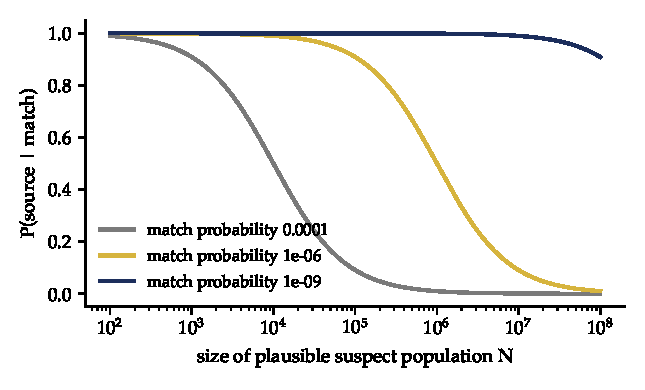
\includegraphics[width=\linewidth]{fig_population}
\caption{Probability that a person who matches a crime stain is its source, as a function of the number of possible sources, with a uniform prior and no other evidence. The prosecutor's fallacy consists in reading the match probability as the probability of innocence.}
\label{fig:population}
\end{figure}

\subsection{The defence fallacy}

The mirror image error is the defence fallacy (Thompson and Schumann's "defense attorney's fallacy"). Counsel argues that since ten people in the city match, the match shows only that the defendant is one of ten, and so it is nearly worthless. This ignores that the match has moved the defendant from being one of ten million to one of ten, a likelihood ratio of a million. Combined with substantial other evidence, such as being seen near the scene, the posterior may become high; with odds of one to ten after the match, other evidence with a likelihood ratio of about a hundred is needed to reach odds of ten to one. The match is highly relevant even though it is not conclusive by itself.\index{defence fallacy}

\subsection{The independence fallacy: People v Collins}

In 1964 a woman in Los Angeles was robbed by a young woman with a blond ponytail who fled in a yellow car driven by a black man with a beard and moustache. The prosecutor in \emph{People v Collins} called a mathematics instructor and invited him to assume probabilities for each characteristic: one in ten for a yellow car, one in four for a man with a moustache, one in ten for a girl with a ponytail, and so on. Multiplying gave one in twelve million, which the prosecutor presented as the probability that a randomly chosen couple would share all the features. The jury convicted. The Supreme Court of California reversed in 1968 \citep{collins1968}. The probabilities had no evidential foundation; the multiplication assumed independence between characteristics that are plainly correlated, such as a beard and a moustache; and even if the figure had been right, it was the probability of a random match, not the probability of innocence. The court's appendix computed, under the prosecutor's own assumptions, that the probability of at least one other matching couple in the Los Angeles area was substantial.\index{People v Collins}

\begin{casebox}{The Collins appendix}
Let $\gamma$ be the probability that a random couple has all the features and $N$ the number of couples in the area. Given that at least one couple matches, the probability that at least two match is
\[
\frac{1 - (1-\gamma)^N - N\gamma(1-\gamma)^{N-1}}{1 - (1-\gamma)^N}.
\]
With $\gamma = 1/12{,}000{,}000$ and $N = 12{,}000{,}000$, this is about $0.42$. Even on the prosecution's numbers, there was a good chance that the couple in the dock was not the only couple in the city that fitted the description.
\end{casebox}

\subsection{Sally Clark}

Sally Clark, an English solicitor, was convicted in 1999 of murdering her two infant sons, who had died suddenly in 1996 and 1998. A paediatrician testified that the chance of two sudden infant deaths in a family like hers was about one in seventy three million, obtained by squaring an estimate of one in 8{,}543 for a single death in an affluent non smoking family. The Royal Statistical Society wrote to the Lord Chancellor to point out the errors. Squaring assumed independence, ignoring genetic and environmental factors shared within a family. More fundamentally, the rarity of two cot deaths says nothing directly about guilt, because double infant murder is also extremely rare. What matters is the ratio of the two probabilities. Ray Hill's analysis of the data suggested that, conditional on two sudden deaths, the odds of natural causes against murder were between about 4.5 to 1 and 9 to 1 in favour of natural causes \citep{hill2004}. The conviction was quashed in 2003, after it emerged that the pathologist had withheld microbiological evidence that one child had a serious infection \citep{clark2003}. Sally Clark died in 2007. Her case is the clearest modern example of a prosecutor's fallacy and an independence fallacy combined, and of the human cost of statistical error.\index{Sally Clark}\index{R v Clark}

The correct comparison is between two rare events. Let $M$ denote double murder and $S$ double sudden infant death, and let $D$ be the observation that both children died suddenly with no obvious cause. Then
\[
\frac{\Prob(M \given D)}{\Prob(S\given D)} = \frac{\Prob(D\given M)}{\Prob(D \given S)} \cdot \frac{\Prob(M)}{\Prob(S)} .
\]
The first ratio may be close to one, since both explanations predict the observation. The second is the ratio of base rates, and on the available data the base rate of double sudden infant death exceeded that of double infant homicide. The figure of one in seventy three million was a poor estimate of $\Prob(S)$, and even a sound estimate of $\Prob(S)$ says nothing until it is set against $\Prob(M)$.

\section{R v Adams: Bayes in front of the jury}

Denis Adams was charged with a rape committed in 1991. The only evidence linking him to the crime was a DNA match, with a reported match probability of one in two hundred million. Everything else pointed the other way. The victim did not pick him out at an identification parade and said he did not resemble her attacker. He was older than the man she described. His girlfriend gave him an alibi. The defence called Peter Donnelly, a professor of statistics, to explain to the jury how to combine the evidence using Bayes' rule, with a questionnaire that led jurors through the calculation for their own chosen numbers \citep{donnelly2005}.\index{R v Adams}\index{Donnelly, Peter}

Adams was convicted. On appeal in 1996 the Court of Appeal ordered a retrial \citep{adams1996}, but it was hostile to the use of Bayes' theorem, saying that it trespassed on the jury's task of evaluating evidence as a whole. At the retrial the defence again led the jury through the method; Adams was again convicted; and on the second appeal in 1997 the Court of Appeal said that the method should not be used in a jury trial without special reason, while offering no alternative account of how the jury should combine the DNA evidence with the rest \citep{adams1998}.

The Adams calculation is worth doing. Suppose the pool of possible offenders is the adult male population within a plausible distance, perhaps one hundred and fifty thousand men. With a uniform prior the prior odds are about $1$ to $150{,}000$. The DNA likelihood ratio, taken at face value, is $2\times 10^8$, which raises the odds to about $1{,}300$ to $1$. The failure of the victim to identify Adams might have a likelihood ratio of around one in nine; the alibi, if given moderate weight, perhaps one in four. Together these give a factor of one in thirty six, bringing the odds to about $37$ to $1$, or a posterior probability of about $0.97$. With a larger pool, a weaker DNA likelihood ratio once laboratory error is considered, or stronger defence evidence, the posterior falls quickly below any plausible criminal threshold, as Figure~\ref{fig:adams1} shows. The point is not that Adams was innocent. The point is that the conclusion depends on judgments the jury was entitled to make, and that without the arithmetic it had no way to see how much those judgments mattered.

\section{R v Doheny and the guidance on DNA}

In \emph{R v Doheny and Adams}, decided in 1996 (reported in 1997; Gary Adams, a different Adams from the case above), the Court of Appeal gave guidance on presenting DNA evidence that is, on its face, Bayesian \citep{doheny1997}. The expert should explain the random match probability and may say how many people in the United Kingdom, or in a relevant subpopulation, would be expected to share the profile. The judge should direct the jury that if, say, four or five people in the country share the profile, the question is whether they are satisfied, in the light of all the evidence, that the defendant is the one who left the stain. This is the island problem expressed in words. The court accepted the logic of the likelihood ratio while rejecting the formula.\index{R v Doheny}

\section{R v T and the limits of likelihood ratios}

In \emph{R v T}, a 2010 murder appeal, the issue was footwear marks. The prosecution's expert had used a likelihood ratio approach, drawing on a database of shoe distribution data to estimate how common the pattern was, and had expressed his conclusion on a verbal scale corresponding to a likelihood ratio at the top of the moderate band (about a hundred). The Court of Appeal held that the likelihood ratio should not be used for footwear evidence where there was no reliable statistical basis for the underlying frequencies, and that the expert's report had not been transparent about how the conclusion was reached \citep{rvt2010}. Forensic statisticians responded that the court had misunderstood the role of the likelihood ratio, which is a framework for reasoning rather than a claim about the precision of the inputs, and that any expert opinion on the significance of a match implicitly makes the same comparison \citep{berger2011}.\index{R v T}

Both sides have a point. The court was right that numbers with no foundation should not be dressed in the authority of calculation, which was the lesson of \emph{Collins}. The statisticians were right that the alternative, an unquantified opinion that a mark could have been made by the shoe, hides the same reasoning without making it better. The constructive response is to require that every likelihood ratio presented in court come with an account of its inputs and their uncertainty, and that experts report ranges where the inputs are soft. We develop this in Chapter~\ref{ch:bf}.

\section{Relevance as a likelihood ratio}

The English law of evidence defines relevance loosely. In \emph{DPP v Kilbourne} Lord Simon said that evidence is relevant if it is logically probative or disprobative of some matter requiring proof \citep{kilbourne1973}. Rule 401 of the United States Federal Rules of Evidence says that evidence is relevant if it has any tendency to make a fact more or less probable than it would be without the evidence, and the fact is of consequence in determining the action. Both definitions have a natural Bayesian reading. Evidence $E$ makes $\Hp$ more probable exactly when $\LR(E) > 1$ and less probable when $\LR(E) < 1$. Irrelevant evidence is evidence with likelihood ratio one.\index{relevance}

This reading clarifies several doctrines. Evidence of a defendant's bad character is relevant if people who commit crimes of the kind charged are more likely to have such a history than people who do not. It may nonetheless be excluded because its probative value is outweighed by prejudice, which in Bayesian terms means, in part, that the jury is likely to overweight it, treating a likelihood ratio of three as if it were three hundred. The exclusionary rule then becomes a correction for a predictable cognitive error rather than a claim that the evidence is irrelevant.

Lord Hoffmann put the general point memorably in \emph{Re B (Children)}: if a legal rule requires a fact to be proved, a judge must decide whether or not it happened, and there is no room for a finding that it might have happened \citep{reb2008}. The law operates a binary system in which the only values are zero and one. The Bayesian reading is that the fact finder forms a posterior probability, compares it to a threshold, and then treats the fact as established or not for the purposes of the legal consequence. The binary system is about the decision, not about the belief.

\section{The weight of evidence as a sequential test}

Turing's use of the weight of evidence at Bletchley was sequential. Each new intercept added weight, and the decision to act was made when the cumulative weight crossed a threshold. Wald's sequential probability ratio test, developed at the same time in the United States, has the same structure. A trial can be read the same way. Each witness, each document, each forensic report adds a weight, positive or negative, and the verdict is reached when the total crosses a threshold. Figure~\ref{fig:decibans} shows simulated paths of cumulative weight for a guilty and an innocent defendant.\index{sequential test}

\begin{figure}[t]
\centering
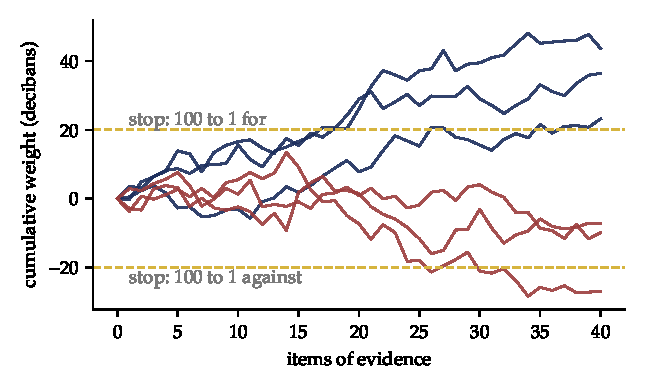
\includegraphics[width=\linewidth]{fig_decibans}
\caption{Simulated paths of cumulative weight of evidence in decibans. Paths generated under guilt drift upward (blue in the digital edition), paths generated under innocence drift downward (red). The dashed lines mark thresholds of twenty decibans, a factor of one hundred.}
\label{fig:decibans}
\end{figure}

The sequential view explains features of trial procedure. The prosecution goes first because it bears the burden; if the weight it adds does not reach a minimum, the judge may withdraw the case from the jury on a submission of no case to answer. The defence then adds its evidence, which typically has negative weight. The jury does not stop part way, because the rules require it to hear everything, but the order in which evidence is heard affects how people weigh it, and much of the craft of advocacy is about sequencing.

The additivity of weights holds only when items are conditionally independent. When they are not, as when two witnesses spoke to each other before testifying, or when a confession and the physical evidence both derive from a police theory, adding weights double counts. Graphical models, the subject of Chapter~\ref{ch:graphs}, are the tool for keeping track of dependence.

\section{Verbal scales and their dangers}

Where juries are not given numbers, as is usual for evidence other than DNA, forensic scientists in England and elsewhere often report likelihood ratios on a verbal scale: weak support, moderate support, moderately strong support, strong support, very strong support, extremely strong support, each corresponding to a range of likelihood ratios. The guidance of the European Network of Forensic Science Institutes is an example. Verbal scales have two dangers. People interpret the same phrase differently, so that strong support may be heard as almost conclusive by one juror and as fairly weak by another. And the phrases describe the evidence, not the hypothesis, but are easily heard as statements about guilt. Research on how lay people interpret such phrases shows wide variation, and some studies find that weak verbal expressions of inculpatory evidence can lower, rather than raise, belief in guilt. A reasonable compromise is to report the number and the phrase together, with an explanation that the number says how many times more probable the evidence is under one account than under the other, and with a reminder that it does not say how probable either account is.

\section{Bayes and the lay fact finder}

Experimental work on juries suggests that people are not hopeless Bayesians. They often update in the right direction, but by too little when evidence is statistical and by too much when it is vivid. Kahneman and Tversky's work on base rate neglect is directly relevant: told that a cab in a hit and run accident was identified as blue by a witness who is right eighty per cent of the time, in a city where fifteen per cent of cabs are blue, most people put the probability that the cab was blue near eighty per cent, while Bayes' rule gives about forty one per cent \citep{tversky1982}. The legal system's response to these biases is partly procedural, through rules of exclusion and judicial directions, and partly structural, through the use of professional judges, appellate review and reasons. A Bayesian analysis can inform each of these responses by identifying where the biases are likely to bite.\index{base rate neglect}

\begin{keybox}
The cab problem. Let $B$ be the event that the cab was blue and $W$ that the witness says blue. With $\Prob(B) = 0.15$, $\Prob(W\given B) = 0.8$ and $\Prob(W\given \bar B) = 0.2$,
\[
\Prob(B\given W) = \frac{0.8\times 0.15}{0.8 \times 0.15 + 0.2 \times 0.85} = \frac{0.12}{0.29} \approx 0.41.
\]
The likelihood ratio of the testimony is four, and the prior odds are about $0.18$, so the posterior odds are about $0.71$.
\end{keybox}

\section{The blue bus and naked statistics}

In \emph{Smith v Rapid Transit}, a Massachusetts case from 1945, the plaintiff was forced off the road at night by a bus she could not identify. The defendant company operated the only franchised bus line on that street. The court held that this was not enough: the probability that the bus belonged to the defendant might be high, but a verdict must rest on actual belief, not on a mathematical chance \citep{smith1945}. Philosophers have built a large literature on the hypothetical in which eighty per cent of the buses in a town are blue and belong to one company. Should a plaintiff hit by an unidentified bus recover against that company on the balance of probabilities? Many philosophers have argued that naked statistical evidence is inherently insufficient.\index{blue bus problem}\index{naked statistical evidence}

The Bayesian analysis distinguishes three issues. The first is whether the statistic is the right prior. Eighty per cent of buses is not the same as eighty per cent of buses on that road at that hour, and the plaintiff who has done no more is presenting a weak prior with no likelihood ratio at all. The second is the incentive effect. If plaintiffs could recover on market share alone, the dominant company would bear liability for its competitors' negligence, and neither firm would have the right incentive to take care. The third is the effect on investigation. A rule that rewards naked statistics discourages the collection of individual evidence, whose expected value of information may be large. Each of these is a reason, in decision theoretic terms, for refusing liability on naked statistics, and none of them requires the claim that statistical evidence is not evidence. Chapter~\ref{ch:standards} takes up the related gatecrasher problem and its solution by expected utility.

\section*{Notes and Questions}
\addcontentsline{toc}{section}{Notes and Questions}
\begin{enumerate}[label=\arabic*.]
\item Show that if $\LR(E) = 1$ then $\Prob(\Hp\given E) = \Prob(\Hp)$ for every prior. Show conversely that if the posterior equals the prior for some prior strictly between zero and one, then $\LR(E) = 1$.
\item In the island problem with $N = 10^6$ and $\gamma = 10^{-6}$, compute the posterior probability that the matching defendant is the source. Suppose a second, independent trait with frequency $1/50$ is also shared. What is the new posterior?
\item Reproduce the calculation in the Collins casebox. Then suppose the true frequency of the combination was one in a hundred thousand. How does the conclusion change?
\item In the Sally Clark case, suppose the probability of a second sudden infant death given a first is one in a hundred rather than one in 8{,}543. Recompute the probability of two deaths in such a family. What does this imply about the independence assumption?
\item Write down a defence argument in the style of \emph{Adams} for a case with a DNA likelihood ratio of $10^7$, a pool of $500{,}000$, a failed identification with likelihood ratio $1/5$, and an alibi with likelihood ratio $1/3$. What is the posterior probability of guilt?
\item Find an example of evidence that is relevant under Rule 401 but would plausibly be overweighted by a jury. Describe a direction that might correct the bias.
\end{enumerate}

\section*{Further reading}
Aitken and Taroni \citep{aitken_taroni2004} and Evett and Weir \citep{evett1998} are standard. Balding's book on DNA evidence is clear and careful \citep{balding2005}. Donnelly's account of \emph{Adams} \citep{donnelly2005} and Hill's analysis of cot deaths \citep{hill2004} reward close reading, and both are collected in Kadane's casebook \citep{kadane2008}.
